\documentclass[11pt,a4paper]{article}
\usepackage[utf8]{inputenc}
\usepackage[english]{babel}
\usepackage{amsmath}
\usepackage{amsfonts}
\usepackage{amssymb}
\usepackage{graphicx}
\usepackage{fancyhdr}
\usepackage{color}
\usepackage{listings}
\usepackage{times}

\pagestyle{fancy}
\lstset{
basicstyle=\footnotesize, 
breaklines=true
}
\begin{document}
\begin{titlepage}
\begin{center}

\includegraphics[width=0.15\textwidth]{UCL.png}
\vfill
\hrulefill
\\[1.2cm]
\textsc{\LARGE LINGI2252 Assignment 2 report}\\[1.2cm]
\hrulefill
\vfill
\begin{minipage}{0.4\textwidth}
\begin{flushleft} \large
Group 17\\
Xiao \textsc{Xu}\\ Xavier \textsc{Crochet}
\end{flushleft}
\end{minipage}
\begin{minipage}{0.4\textwidth}
\begin{flushright} \large
Kim \textsc{Mens} \\
Sergio \textsc{Castro} \\
\end{flushright}
\end{minipage}
\vfill

\includegraphics[width=0.30\textwidth]{EPL.jpg}\\
\vfill
\end{center}
\end{titlepage}


\tableofcontents
\newpage
\section{Introduction}
In the first report, we try to do a manual analysis of \textit{Glamour}. This first step gives us a global overview of \textit{Glamour} and helps us to understand how \textit{Moose} and his tools work. Because of the size of the system (about 270 classes), we use some tools in order to get some hints on where to begin. It wasn't exactly what was asked in the statement of the first report but now that we have all the tools in our hand, we can start looking more effectively for the needles in the haystack that \textit{Glamour} is.\\

Moreover, we found some code duplication in the source code (but relatively few compared to the size of the framework) and the utilisation  of the \textit{Pattern Observer} in the \textit{GLMPresentation} class. We thus conclude that \textit{Glamour} was globally well-designed, despite the few code duplication.\\

The report will be divided into two parts:\\
\begin{enumerate}
	\item We start by analysing the code using criteria not identifiable by metrics to see
		\begin{itemize}
		\item How well the code is commented.
		\item How good the naming convention is.
		\end{itemize}
	\item Then, we develop a set of metrics we'll use later to analyse the code to identify the attributes causing the elephant classes.
\end{enumerate}
\newpage

\section{Architecture}
\subsection{Overview Pyramid}
With moose, we can easily have a pyramid visualisation of the system.\\
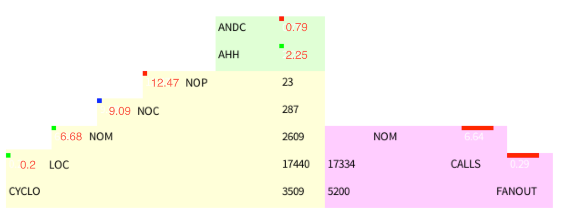
\includegraphics[width=\textwidth]{pyramid}

As you can see, three different colours are used in the figure.
\begin{enumerate}
\item The \textcolor{green}{green} part provides information about the depth of the inheritance. \textit{ANDC} means "Average number of derived classes" and \textit{Average Hierarchy height}.  
\item The \textcolor{yellow}{yellow} part provides information about the complexity of the system. \textit{NOP} means number of package, \textit{NOC}, number of classes, \textit{NOM}, number of methods, \textit{LOC}, lines of code and \textit{CYCLO}, cyclomatic number.
\item In \textcolor{magenta}{purple} part provides information about coupling. \textit{NOM} means number of methods, \textit{CALLS}, number of invocation and \textit{FANOUT}, number of called classes.
\end{enumerate}

On the left top of each pyramid component, there is a small coloured dot.
\begin{itemize}
\item \textcolor{green}{Green} means good.
\item \textcolor{blue}{Blue} means average.
\item \textcolor{red}{Red} means bad.
\end{itemize}

From this picture, we made some observations. 
\begin{itemize}
\item It seems that glamour behaves quite good in term of complexity.
\item Their is some use of hierarchy, but the average number of derived classes is quite low.
\item The coupling part is very bad. 
\end{itemize}

This figure gave us some leads on where to begin our analysis.  
\subsection{Complexity}
In the first report, we print the whole figure displaying the system complexity. We conclude they were some elephant classes with a lot of methods in the system.  
\section{Comments}
Commenting code is important to improve \textbf{readability} and  the \textbf{re-usability}. It makes it easier for developers to continue a project or for student to analyse it.\\

There are so few comments in the code that we decide to not use a metric to analyse this part. In deed, there are only 768 comments! That's about 3 comments for each class.
\section{Naming Convention}

A good naming convention is also an important point in order to improve \textbf{readability} and \textbf{re-usability} of the code. Using the \textit{Name Cloud} utility from moose, we can display the following figure, showing the most used words \textbf{for naming classes} in the framework.\\
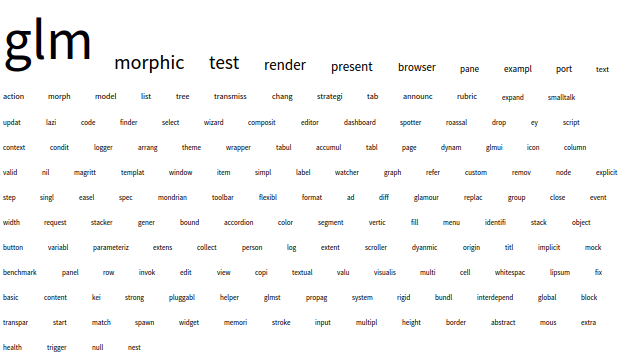
\includegraphics[width=\textwidth]{name_cloud}
\\
As we can see \textbf{GLM} is the suffix coming up the more often. Other suffix such as \textbf{test} \textbf{render} or \textbf{morphic} arise too. It seems that classes are named quite correctly in order to provide meta-information about their use.\\

We can perform the same analysis for methods or variable.Globally there is no bad smells coming up here. There is not randomly named classes variable or methods. Anyway, naming convention is quite a controversial issue, so we are not going deeper in the analysis here. 
\section{Metrics-based analysis}
\subsection{Introduction}
Before deciding when to re-factor, we need first to identify where bad smells occurs inside the framework. Using \textit{Moose}'s metrics set, we start by establishing criteria to identify those parts.\\ 

In practice, we'll use the following query in order to retrieve the classes based on our pair of metrics-threshold:\\

\begin{lstlisting}
((self flatCollect:[:each | each classes]) flatCollect:[:each | each methods]) select:[:each | (each ATTRIBUTE OPERATOR THRESHOLD)] 
\end{lstlisting}

If we want only to look into classes, we can do:\\
\begin{lstlisting}
(self flatCollect:[:each | each classes])  select:[:each | (each ATTRIBUTE OPERATOR THRESHOLD)]
\end{lstlisting}
%(MooseModel root allModels first) allClasses select: [:each | (each METRICNAME OPERATOR THRESHOLD)]
Avec
\begin{itemize}
\item ATTRIBUTE - The name of the attribute
\item OPERATOR - The operator for the comparison
\item THRESHOLD - The value of the threshold
 \end{itemize}

When we wrote the first report, it appears clearly that they was some big classes in the code. We'll start by using \textit{Elephant-identifiers} attributes such as:
\begin{itemize}
\item Cohesion
\item Code Duplication
\item Large Method and Classes
\end{itemize}

to try to explain what goes wrong inside these classes (and propose solutions).  
\subsection{Elephant-identifier attributes}
\subsubsection{Code duplication}
Having the same code structure in more than one place in the system is quite nasty. The program will be better if we find a way to reunite them.The attributes we have to handle are \textit{NumberOfExternalDuplications} and \textit{NumberOfInternalDuplications}.\\

\textbf{Threshold} - \textit{SmallDude}, the tool used by moose to detect duplicated code have a threshold of 3 lines. We decide here to set the threshold of the two attributes to 0, and to analyse one at the time the results.\\

When querying for
\begin{itemize}
\item \textit{NumberOfInternalDuplications} we get 27 classes
\item \textit{NumberOfExternalDuplications} we get 30 classes
\end{itemize}
Let's take for example the class \textit{GLMBasicExample}.
\begin{itemize}
\item We have 3 external duplications, meaning that we have 3 block of code present in three other class of the framework. The duplication with \textit{GLMUpdateInterdepententPanesTest} is the following:
\begin{lstlisting}
browser := GLMTabulator new.
browser
	column: #one;
	column: #two;
	column: #three.
(browser transmit)
	to: #one;
	andShow:[:a] a tree display:[:x|1 to: x]].
(browser transmit)
	to: #three;
	from: #two;
\end{lstlisting}
here, we can extract a new class from \textit{GLMBasicExample} and use it inside \textit{GLMUpdateInterdepententPanesTest}.

\item We have also 6 internal duplications. The following piece of code is present two times in the class.
\begin{lstlisting}
|browser model|
	model := Dictionary new.
	model at: #some put: #(1 2 3 4).
	model at: #even put: #(2 6 8).
	model at: #odd put: #(3 7 9).
	
	browser := GLMTabulator new.
	browser column: #one.
	browser transmit to: #one; andShow: [ :a |
		a tree
			display: [model keys];  
\end{lstlisting}

We can re-factor the classes by extracting the duplicated blocks as new methods, making the class more maintainable.\\

Basicly, the solution is to \textbf{extract} the duplicated block as \textbf{a new method} when  an internal one occurs, and as a \textbf{new class} when it's an external. When a external duplicated block occurs between \textbf{two parent classes}, it's more appropriate to resolve it using \textbf{inheritance}. 
\end{itemize}	
\subsubsection{Cohesion}
Cohesion metrics measure how well the methods of a class are related to each other. A cohesive class performs one function. A non-cohesive class performs two or more unrelated functions. The idea is to re-factor the non-cohesive class into several smaller classes. Cohesion is thus a good thing.

The attribute to inspect here is \textit{tightClassCohesion}. It's a ratio between number of connected methods and the maximum number of possibly connected methods. Two methods are connected if they access the same attribute. 
We modify our query a little bit:
\begin{lstlisting}
(self flatCollect:[:each | each classes])  select:[:each | ((each tightClassCohesion  >= MIN) &( each tightClassCohesion < MAX))]
\end{lstlisting}

And compute the following graph, displaying the number the repartition of all the classes in term of their cohesion value.\\
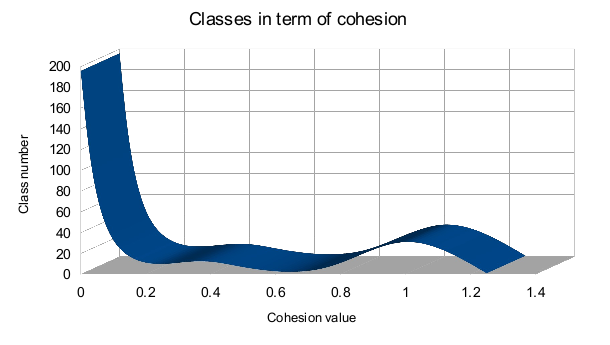
\includegraphics[width=\textwidth]{cohesion_result}

\begin{itemize}
\item We see thaht the class having the highest cohesion value (1.47) is \textit{GLMUpdateMorphicTest} and has only \textbf{96 lines of codes}.\\

\item About ~200 classes have less than O.1 cohesion. 
\end{itemize}

\begin{minipage}[t]{0.4\textwidth}
When we ask moose to display the concerned classes, we see that the concerned classes are the elephant one of the framework. Furthemore, the whole \textit{GLMPresensation} Family appears on the picture (as you can see in the picture to the right):

\end{minipage}
\hfill
\begin{minipage}[t]{0.6\textwidth}
    \centering
     \vspace{-1.5ex}
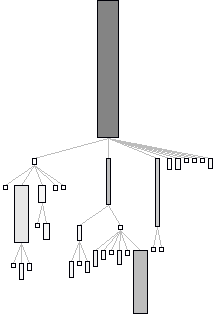
\includegraphics[width=0.6\textwidth]{GLMPresentation_family}
\end{minipage} 


Theses classes (\textit{GLMPresentation}, \textit{GLMCompositePresentation} \textit{GLMListingPresentation}, \textit{GLMWizard}, \textit{GLMBrowser}, ...)  where also identified in the first report as elephant  classes.\\
\subsubsection{Coupling}
Coupling measures the interdependence of class with other classes. Tight coupling is a bad thing. It reduces flexibility and re-usability while increasing the difficulty to implements test. In order to measure coupling, we use the following metrics:
\begin{itemize}
\item \textit{fanIn} : The number of classes referencing our class.
\item \textit{fanOut} : The number of classes referenced by our class.
\end{itemize} 

We 
\begin{itemize}

\item Compute the following metric:
$tightClassCoupling = \frac{fanOut}{fanIn}$

It measure the tightness of a class's cohesion.
\item Use the following query
\begin{lstlisting}
(self flatCollect:[:each | each classes])  select:[:each | 
	(
	(each fanIn  > 0)  
	ifTrue: 
	[
	(each fanOut / each fanIn) < THRESHOLD_VALUE
	]
	ifFalse:  [ false ]
	)
]
\end{lstlisting}
Some classes have a \textit{fanIn} attribute whose value is zero. To overcome this issue, we decide to ignore theses classes. In deed, after querying for them, we found out that all those classes were test ones. That explains why there aren’t called by any other classes. 

\item{Compute the following graph with the collected data.}
\end{itemize}

 
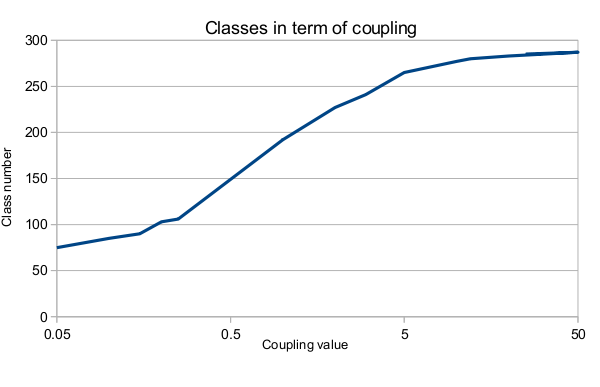
\includegraphics[width=\textwidth]{coupling_result}
\textit{Note : We use a logarithmic scale to display the x axis.}\\

Immediately, it appears that, if we invert the x-axis, the curve has the same shape as the cohesion one (See the above section). Once again, all the big classes have high coupling numbers.
\subsubsection{Large methods-classes}
To pursue our elephant classes analysis, we can look into these metrics:\\
\begin{tabular}{| c | c | c |}
\hline
Metric & Threshold 1 & Threshold 2\\
\hline
numberOfLinesOfCode & 25 & 30\\
\hline
numberOfStatements & 15 & 25\\
\hline
numberOfMessageSends & 10 & 20\\
\hline
\end{tabular}\\
The idea here is to look for classes having large methods doing a lot of stuff. So we look for method respecting the following rule:

\begin{quote} $ numberOfLinesOfCode > 25 \\ \vee numberOfStatements > 15 \\ \vee numberOfMessageSends > 10$\\\end{quote}

We get 196 classes. If we look at the complexity graph, these are the same classes we get on the above section. To be certain, we increase our threshold (See the second threshold of the table). We get 150 classes, among them, the one we identify in the first report and in the previous section.
\subsubsection{Long list parameters}
Overloading method declaration with a lot of parameters quickly turns the code hard to understand, making it inconsitend and difficult to use. In deed, a good practice is to get information through object request, rather than using parameters.\\

Using the \textit{numberOfparameters} attribute,  we see that there are only 20 classes with more than 5 parameters here. But among the corresponding methods, half of them belong to \textit{GLMPresentation} class (our evil class).
\subsubsection{Accessors}
There are different ways to access an attribute:
\begin{itemize}
\item Using an accessor/mutator.\\ This is the best way in the oriented-object programming. According to this principle, the attribute is made private to hide and protect it from other code. It can neither be used directly, nor e modified by other code, except by the accessor/mutator function.
\item Directly from outside of the class. \\ This is dangerous, and could cause some maintenance problems, because we are limited to modify the code
\item Directly from inside. \\ This is not good too, but this will not be a big problem if they are accessors/mutators inside the class and we have just forgotten to use them. The reason is that, for the person who maintains the code, he just needs to take care of the code inside the class.\\ However, if there isn't any accessors/mutators, it will clearly become and issue. The person maintaining the program must not only check this class, but also find out all the uses/modifications of the attribute.
\end{itemize}

We consider that, for a good class, every attribute has one \textit{getter} method (accessor) and on \textit{setter} (mutator) method. Therefore, there are \textbf{two} accessor-methods per attribute.\\

The Glamour system has 287 classes. We fill find out among them how well attribute are accessed.\\

At first, we should know how many classes have attributes by using the following query:\\
\begin{lstlisting}
((self flatCollect:[:each|each classes])
	select:[:each|each numberOfAttributes>0]
\end{lstlisting}
\textbf{Glamour has 138 classes with attributes.}\\
Then we query for classes respecting the following rule:\\
$(numberOfAttributes) > 0) ^ (numberOfAccessorMethods >= (2*each numberOfAttributes))$

This query results in 36 classes that might correctly access their attributes. \textbf{But}, we have to be aware that they might be some attributes with 3 or more accessors-methods. As consequence, they might be some false positives results with attributes having only 1 or 0 accessor method.\\ 

The solution is to query for classes having more than 3 accessor methods and to manually look into them. Luckily, there is only one class printed out:  \textit{GLMPanePort}). The maximum number of well designed classes is thus 36.\\

Therefore, we can compute the proportion of good classes as follow: $\frac{Classes respecting the rule}{Classes with attributes} = \frac{36}{138} = 26.09\%$
 This percentage shows that most of the classes don't access correctly their attributes. However, not all the attributes need an accessor and a mutator, the results might be truncated.\\ 

In order to going deeper, we try to get more information that might help us to further analyse the \textit{Glamour System}. Thus, we query for classes having one or more attributes. There are 78 classes respecting this rule.\\

Therefore, we have 47 classes having attributes without accessor-methods. They could cause maintenance problems.\\

Now, we are going to look for classes accessing directly their attributes. First, we use the following query to get the total number of attributes.
\begin{lstlisting}
((self flatCollect: [:each | each classes]) flatCollect: [:each |each attributes])
\end{lstlisting}
We get 364 attributes.

We can get the number of directly accessed variable using the \textit{numberOfGlobalAccesses} metrics. That represents only $2.20\%$ of the total attributes of the system. That's very nice!

But, using the following query\\
\begin{lstlisting}
((((self flatCollect: [:each | each classes])
	select: [:each | each numberOfAttributes > 0])
	select: [:each | each numberOfAccessorMethods > 0]))
flatCollect: [:each | each attributes])
select: [:each | numberOfGlobalAccesses > O ]
\end{lstlisting}
it appears that, among these 8 attributes, 4 of these globally acceded attributes have accessor-methods!\\

We can compute the following chart, showing information about class using accessor-methods:\\
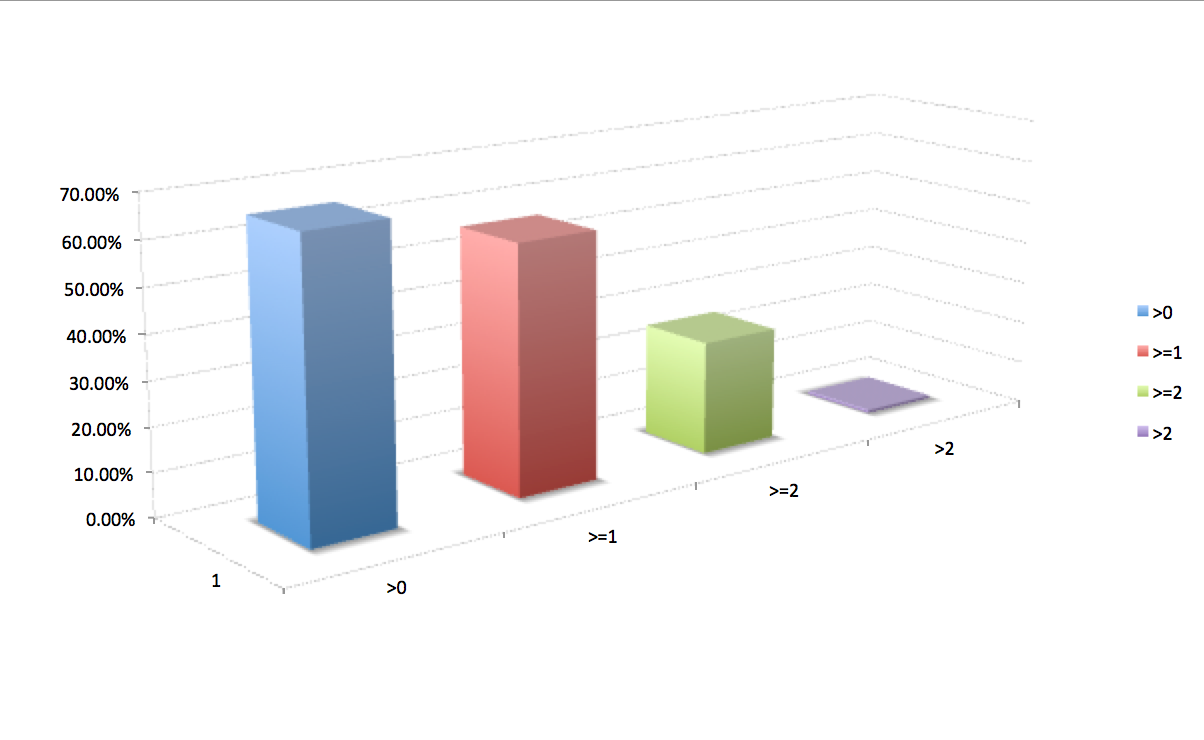
\includegraphics[width=\textwidth]{accessor.png}
\begin{itemize} 
\item The \textcolor{blue}{blue} column represents classes having accessor-methods (about 66\%)
\item The \textcolor{red}{red} one represents classes having at least one accessor-method (about 57\%)
\item The \textcolor{green}{green} one represents the \textit{good} classes (about 26\%)
\item The \textcolor{magenta}{purple} one represents having 2 or more accessor-methods for only one attribute. (Only one class)
\end{itemize}
There are many classes with no accessor-methods, which will may cause maintenance problems in the future. Furthemore, we see that they might be some false-positives, as they might be an average of 2 accessor method per attribute if one atribute has only one accessor and an other 3. But, as there are only 8 directly acceded attributes, we see that the developer rarely use such bad smells.  


\subsubsection{Conclusion}
If we query for classes having low cohesion, high coupling, high line number of code and large methods, we get always. similar results. Even more, we reach one of our first report conclusion (We identified a large number of big classes.) We come up here the first design problem of the framework: \emph{Cohesion}. One must increase the cohesion of theses classes by re-factoring them into smaller ones.\\

Some of the concerned classes are:\\ 

\begin{tabular}{| c | c | c | c | c |}
\hline 
\textbf{Class Name} &\textbf{ Lines of code} & \textbf{Messages sent} & \textbf{Cohesion} & \textbf{Coupling}\\
\hline
GLMBasicExample & 1370 & 1600 & 0.0 & 3.9565\\
\hline
GLMPresentation & 659 & 502 & 0.076 & 2.6093\\
\hline
GLMWhiteSpaceTheme & 778 & 524 & 0.0 & 4.25 \\
\hline
GLMUITheme & 797 & 552 & 0.0 & 4.7272\\
\hline
GLMCompositePresentation & 255 & 287 & 0.0051 & 0.4659\\
\hline 
GLMWizard &  374 & 321 & 0.0029 & 1.6206\\
\hline
GLMBrowser & 360 & 436 & 0.012 & 0.8041\\
\hline
\end{tabular}
\section{Improvements}
\section{Conclusion}
\end{document}
